\chapter{Web Ontology Language} \label{ch:owl}

By adding schema to RDF, RDFS already boosts the capability and adds ontology to the RDF model. As demonstrated in the previous chapter, RDF/RDFS is able to process simple logic reasoning. However, RDF/RDFS alone cannot handle DL. OWL is, therefore, proposed to enable DL in the semantic web.

Notice that it is OWL the abbreviation of web ontology language, not WOL, for historical contexts reasons.

\section{RDF/RDFS Limitations} \label{subsec:rdfrdfslimitations}

Several examples are given to demonstrate the limitations of RDF/RDFS.

RDFS brings schema to the RDF model by introducing class and property hierarchy. For example, in the schematic design of the model we can create ``animal eats food'', where ``eat'' is a property with domain ``animal'' and range ``food''. We can then add instances to animal and food classes. This is demonstrated in Fig. \ref{fig:coweatgrass}. The SPARQL to create such an RDF model is given below.
\begin{lstlisting}
	PREFIX ex: <http://www.example.com/>
	PREFIX rdfs: <http://www.w3.org/2000/01/rdf-schema#>
	PREFIX rdf: <http://www.w3.org/1999/02/22-rdf-syntax-ns#>
	
	INSERT DATA {
		# Define resources
		ex:Human rdf:type ex:Animal .
		ex:Cow rdf:type ex:Animal .
		ex:Vegetable rdfs:subClassOf ex:Food .
		ex:Meat rdfs:subClassOf ex:Food .
		ex:Cabbage rdf:type ex:Vegetable .
		ex:Ribeye rdf:type ex:Meat .
		
		# Define properties
		ex:eat rdf:type rdf:Property ;
		rdfs:domain ex:Animal ;
		rdfs:range ex:Food .
		
		# Define triples
		ex:Human ex:eat ex:Meat .
		ex:Human ex:eat ex:Cabbage .
		ex:Cow ex:eat ex:Cabbage .
	}
\end{lstlisting}

\begin{figure}[htbp]
	\centering
	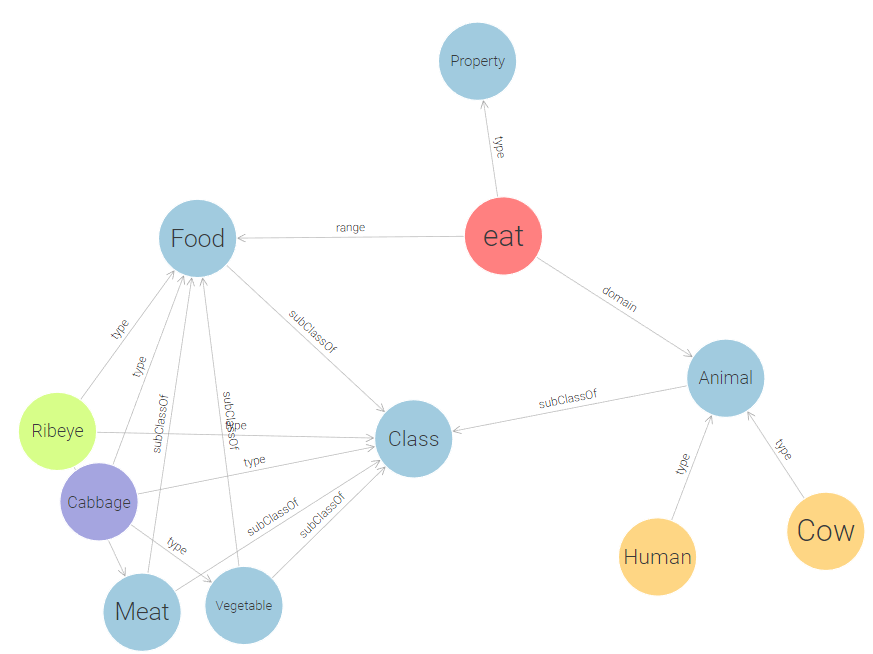
\includegraphics[width=0.8\textwidth]{chapters/part-4/figures/coweatgrass.png}
	\caption{An RDF model that demonstrates ``animal eats food''.}
	\label{fig:coweatgrass}
\end{figure}

From Fig. \ref{fig:coweatgrass}, under OWA when querying what animals eat what food, the following would be returned:
\begin{itemize}
	\item Human eats rib-eye.
	\item Human eats cabbage.
	\item Cow eats rib-eye (this is not what we expect).
	\item Cow eats cabbage.
\end{itemize}
Since it is not explicitly denied that cow cannot eat meat, under OWA, semantic web thinks that there is the possibility of cows eating meat. RDF/RDFS cannot exclude meat from the menu of a cow, or to say it in general, RDF/RDFS cannot add restrictions to a property.

A walk around is to define two properties, ``eatMeat'' and ``eatVegetable'', each with their associated ranges. Let human have both properties while cow have only ``eatVegetable'' property. However, this complicates the connection of symbols and destroys the schema of the model, essentially making null the effort of RDFS.

Similarly, consider an example where ``hasVisualAcuity'' is used to describe human's clarity of vision. A person usually have two visual acuity values for the two eyes. In RDF, that means a person should have two and only two ``hasVisualAcuity'' property. This cannot be enforced by RDF/RDFS.

Consider another example where ``man is a subclass of human'' and ``woman is a subclass of human''. With only RDF/RDFS, however, there is no way to add restrictions that says ``a person cannot be man and woman at the same time'', i.e., to disjoint man class and woman class.

RDF/RDFS does not support class combinations. For example, for existing classes ``Car'', ``Motorcycle'', ``Bicycle'', ``Ship'', ``Plane'', RDF/RDFS cannot create a new class ``AllTranportationTool'' to automatically include every instance from the above classes. In general, with RDF/RDFS alone, it is not possible to define a class which is a union/intersect/complement of other classes.

In semantic web stack Fig. \ref{fig:semanticwebstack}, one layer above RDF/RDFS, OWL is proposed to solve the above problems.

\section{OWL Vision}

OWL essentially introduces DL inference to the semantic web, making it more expressive and capable of complicated reasoning. With that in mind, OWL provides additional features to enforce and enhance the schema of an RDF model, thus addressing the problems mentioned in Section \ref{subsec:rdfrdfslimitations}. It allows adding relations and property constraints to the RDF model. The following summarizes the main features introduced by OWL.
\begin{itemize}
	\item Allow the disjoint of sub classes (an instant cannot be man and woman at the same time).
	\item Allow enforcing the number of attributes of each property type (one can have only one social security number, but can have many mail addresses)
	\item Allow enforcing the range of the values an attribute can take (the age of a person must be a positive integer).
	\item Offer more expressive class definitions including union, intersection, complement, etc.
	\item Enlarge the vocabulary sets on top of RDF/RDFS.
\end{itemize}

As of this writing, OWL 2 is the latest version of OWL recommended by W3C. It makes the following assumptions:
\begin{itemize}
	\item OWA. In this context, the knowledge base is considered open, and absence of information must not be valued as negative.
	\item An instance can have non unique names, i.e., multiple syntax can be mapped to the same instance via interpretation.
\end{itemize}

In practice, OWL comes in different flavors, including OWL Lite, OWL DL and OWL Full, just to name a few. OWL 2 supports different choices of syntax, including RDF-syntax, XML-syntax, functional-syntax, Manchester-syntax, and Turtle.

\section{OWL Basic Syntax}

Unless otherwise mentioned, Turtle is used when introducing OWL syntax. Classes, individuals, and properties are already introduced in RDF/RDFS. OWL also defines these concepts, each with enriched features. It is worth mentioning that OWL defines two special classes, \verb|owl:Thing| and \verb|owl:Nothing|, corresponding with the top class (universal set) and bottom class (empty set) in DL, respectively.

\vspace{0.1in}
\noindent \textbf{Class and Subclass}
\vspace{0.1in}

Defining a class from the root \verb|owl:Class| using OWL is given below.
\begin{lstlisting}
	:Fruit a owl:Class ;
\end{lstlisting}
where \verb|a| can be replaced by \verb|rdf:type|. To define an individual via class membership, simply use
\begin{lstlisting}
	:Apple a :Fruit .
\end{lstlisting}
which is equivalent of saying \verb|Fruit(Apple)| in DL. It is also possible to define an individual without a named class as follows, which indicates that the named class will be added in a later stage. In this case, \verb|owl:NamedIndividual| is used.
\begin{lstlisting}
	:ANewThing a owl:NamedIndividual .
\end{lstlisting}

Subclass can be defined similarly as follows.
\begin{lstlisting}
	:Fruit a owl:Class ;
	rdfs:subClassOf :Food .
	:Meat a owl:Class ;
	rdfs:subClassOf :Food .
	:Food a owl:Class .
\end{lstlisting}

Notice that it was impossible to enforce class disjoint using RDF/RDFS alone. This is made possible in OWL as follows.
\begin{lstlisting}
	:Fruit owl:disjointWith :Meat .
\end{lstlisting}
Or alternatively,
\begin{lstlisting}
	[] a owl:AllDisjointClasses ;
	owl:members
	(	:Fruit
	:Meat
	:SoftDrink
	:Beer ) .
\end{lstlisting}
which is a shortcut when disjoint is claimed on multiple classes. Similarly, class equivalence can be defined using \verb|owl:equivalentWith| keyword.

\vspace{0.1in}
\noindent \textbf{Property}
\vspace{0.1in}

There are two types of properties defined in OWL, namely the object property which links to another resource URL (another object), and datatype property which links to a literal. Examples are given below.
\begin{lstlisting}
	:hasColor a owl:ObjectProperty ;
	rdfs:domain :Fruit ;
	rdfs:range :Color .
	:hasShelfLife a owl:DatatypeProperty ;
	rdfs:domain :Fruit ;
	rdfs:range xsd:integer .
\end{lstlisting}
where notice that XML schema definition (XSD) defines many data types and sub data types, including \verb|xsd:integer|, \verb|xsd:string|, \verb|xsd:decimal|, \verb|xsd:boolean|, \verb|xsd:date| (a calendar date), \verb|xsd:time| (time in a day), \verb|xsd:dateTime|, \verb|xsd:double| (64-bit floating number), \verb|xsd:float| (32-bit floating number), \verb|xsd:anyURI|, \verb|xsd:language|, etc.

\section{OWL Advanced Syntax}

\vspace{0.1in}
\noindent \textbf{Equivalent and Different Individuals}
\vspace{0.1in}

In RDF/RDFS, different individuals are distinguished by their names, and each individual can have one and only one name (it is technically possible for an individual to have no name, but it is not often a good practice). In OWL, it is possible to either map multiple names to the same individual, or to emphasize that two names are pointing to different individuals (this is sometimes necessary due to the OWA). Examples are given below.
\begin{lstlisting}
	:Computer a owl:Class .
	:HarryPc a :Computer .
	:PotterPc a :Computer ;
	owl:sameAs :HarryPc .
	:DumbledorePc a :Computer ;
	owl:differentFrom :HarryPc .
\end{lstlisting}
To state that individuals are different, alternatively use the following
\begin{lstlisting}
	[] a owl:AllDifferent ;
	owl:distinctMembers
	( :HarryPc,
	:DumbledorePc,
	:HermionePc,
	:HagridPc	) .
\end{lstlisting}

\vspace{0.1in}
\noindent \textbf{Closed Class}
\vspace{0.1in}

It is possible to define an enumerate class, whose instances are taken from individuals. An example is given below.
\begin{lstlisting}
	:Weekdays a owl:Class ;
	owl:oneOf
	(	:Monday
	:Tuesday
	:Wednesday
	:Thursday
	:Friday ) .
\end{lstlisting}
which indicates that any individuals to be defined under class ``Weekdays'' must be one of the 5 individuals ``Monday'', ``Tuesday'', etc. Do not confuse \verb|owl:oneOf| with \verb|owl:unionOf|, as the former defines a class as an enumerate of individuals, and the later defines a class as an enumerate of subclasses.

\vspace{0.1in}
\noindent \textbf{Class Constructors}
\vspace{0.1in}

Intersection, union and complement are the commonly seen class (set) constructors. They can be defined as follows.
\begin{lstlisting}
	:MyFavourateBook a owl:Class .
	:HisFavourateBook a owl:Class .
	:OurFavourateBook a Class ;
	owl:intersectionOf (:MyFavourateBook :HisFavourateBook) .
	:Wine a owl:Class ;
	owl:equivalentClass [
	owl:unionOf (
	:DryWine
	:MediumWine
	:SweetWine
	)
	] .
	:Plant a owl:Class ;
	rdfs:subClassOf [
	owl:complementOf :Animal
	] .
\end{lstlisting}

\vspace{0.1in}
\noindent \textbf{Property Restrictions}
\vspace{0.1in}

It has been introduced earlier that the type of the property can be specified by using either \verb|owl:ObjectProperty| (specify range as a class) or \verb|owl:DatatypeProperty| (specify range as a datatype such as string, decimal, integer, etc). In the context of OWL, more restrictions can be enforced to properties, including the number of appearance of each property, and the values each property can take. Details are given below.

The syntax of adding different property restrictions may differ slightly. A general syntax is given by
\begin{lstlisting}
	:<Class> rdfs:subClassOf [
	rdf:type owl:Restriction ;
	owl:onProperty :<PropertyName> ;
	owl:<RestrictionType> <RestrictionDetails>
	] .
\end{lstlisting}
where the blank node is used for property restrictions.

For example, to indicate that the value of a property must be taken from a class, use
\begin{lstlisting}
	:<Class> owl:restriction [
	owl:onProperty :<PropertyName> ;
	owl:allValuesFrom :<RestrictionClass>
	] .
\end{lstlisting}
And to indicate that among all the property values of a property, at least one of them must take values from a class, replace \verb|owl:allValuesFrom| with \verb|owl:someValuesFrom|.

To indicate that a property must take specific value, use \verb|owl:hasValue| at the restriction type, and put the value as \verb|<RestrictionDetails>|, whether an individual or a datatype value.

To restrict the number of a property, use \verb|owl:maxCardinality|, \verb|owl:minCardinality| or \verb|owl:cardinality|, and put the maximum, minimum or fixed number as \verb|<RestrictionDetails>|.

It is possible to define a class from property restrictions, essentially saying ``the class is defined as a collection of individuals that satisfy the following property restrictions''. To do that, use \verb|rdfs:subClassOf| with property restrictions as given in the example below.
\begin{lstlisting}
	:MyBook a owl:Class ;
	rdfs:subClassOf [
	a owl:Restriction ;
	owl:onProperty :hasOwner ;
	owl:hasValue :Me
	] .
\end{lstlisting}
where \verb|:Me| is a predefined individual that maps to myself. To put it in words, a book is considered an instance of \verb|:MyBook| if it has a \verb|:hasOwner| property with the value \verb|:Me|.

\vspace{0.1in}
\noindent \textbf{Property Hierarchy}
\vspace{0.1in}

Properties can have hierarchy like classes. Properties hierarchy can be realized using \verb|rdfs:subPropertyOf| in RDF/RDFS framework. OWL further enriches that idea, by introducing new concepts such as \verb|owl:inverseOf|. Examples below are used to demonstrate property hierarchy.

To define property hierarchy, use
\begin{lstlisting}
	:isOwnerOf a owl:ObjectProerty ;
	rdfs:subPropertyOf :isMasterOf ;
	rdfs:domain :Person ;
	rdfs:range :Book .
	:isOwnedBy a owl:ObjectProperty ;
	owl:inverseOf :isOwnerOf ;
	rdfs:domain :Book ;
	rdfs:range :Person .
\end{lstlisting}
Notice that when defining a inverse property, it is not necessary, but still good practice, to point out the domain and range. This is for better readability and easier error checking.

OWL further defines the following features of a property.
\begin{itemize}
	\item \verb|owl:TransitiveProperty|: if \verb|Property(a,b)| and \verb|Property(b,c)|, then \verb|Property(a,c)|. An example is ``isAncestorOf''.
	\item \verb|owl:SymmetricProperty|: if \verb|Property(a,b)|, then \verb|Property(b,a)|. An example is ``isColleagueWith''; there is also \verb|owl:AsymmetricProperty|, which indicates that if \verb|Property(a,b)|, it is not possible that \verb|Property(b,a)|.
	\item \verb|owl:FunctionalProperty|: if \verb|Property(a,b)| and \verb|Property(a,c)|, then \verb|b=c|. An example is \verb|hasMother|.
	\item \verb|owl:InverseFunctionalProperty|: if \verb|Property(a,c)| and \verb|Property(b,c)|, then \verb|a=b|. Examples are \verb|isMotherOf|, \verb|hasId| (assuming ID is unique for each individual).
\end{itemize}

Restrictions \verb|owl:disjointWith| and \verb|owl:AllDisjointClasses| can be used to claim disjoint of classes, it is possible to declare disjunctive properties using \verb|owl:propertyDisjointWith| and \verb|owl:AllDisjointProperties| as follows. Disjunctive properties cannot take the same value. For example,
\begin{lstlisting}
	:hasParent a owl:ObjectProperty ;
	rdfs:domain :Person ;
	rdfs:range :Person .
	[] a owl:AllDisjointProperties ;
	owl:members ( :hasParent :hasChild :hasSibling ) .
\end{lstlisting}

In OWL, top and bottom classes are defined, corresponding to the universal set and empty set, respectively. Similar ideas apply to properties. Object and datatype properties each has its top and bottom properties.

It is possible to declare a negative assertion as a property to state that a relation does not hold for two individuals. An example is given below.
\begin{lstlisting}
	[] a owl:negativePropertyAssertion ;
	owl:sourceIndividual :SherlockHolmes ;
	owl:assertionProperty :isMurderOf ;
	owl:targetIndividual :Watson .
\end{lstlisting}
which claims that it is not true that ``SherlockHolmes'' has the property ``isMurderOf'' with the range ``Watson''. Notice that negative assertion is supported only at individual-to-individual level. It is currently not possible to claim that Sherlock Holmes is not a murder of any victims, i.e, \verb|:Watson| cannot be replaced by a class such as \verb|:Person|. In FOL, this would have been possible. But currently OWL does not adopt FOL for a good reason (FOL can be undecidable, and too computationally expensive).

\vspace{0.1in}
\noindent \textbf{General Role Inclusion}
\vspace{0.1in}

If we define ``B is the father of A'' and ``C is the brother of B'', then naturally, ``C is the uncle of A'' can be derived. This role chain can be realized via OWL general role inclusion. However, this adds uncertainty to the reasoning, and may cause the model to be undecidable. This is one of the reasons why different tiers of OWL have been proposed. More features usually mean more computations and higher risks of undecidable results, and the user needs to decide which tier to use.

And do notice that due to the G\"odel's incompleteness theorems, there is no sophisticated enough system or knowledge base that can use finite input to derive all the knowledge in a complete (every statement can be proved true or false) and consistent (no contradiction) way.

Using role chain, we can define \verb|isUncleOf| as follows.
\begin{lstlisting}
	:isUncleOf a owl:ObjectProperty ;
	owl:PropertyChainAxiom ( :hasFather :hasBrother ) .
\end{lstlisting}

It is not recommended ot use role chain in a semantic web.

\section{Semantic Web with Rules}

Rules (rule-based systems, also known as rule-based engines) are used to express logic beyond DL, i.e., beyond what RDF/RDFS and OWL can describe. From this perspective, one can think of rules-based semantic web as a further enhancement beyond RDF/RDFS and OWL.

The basic syntax of a rule is simply
\begin{lstlisting}
	IF A THEN B
\end{lstlisting}
where \verb|A| and \verb|B| are premises and conclusion respectively. There are many variations, including logical rules (FOL rules, for example), procedural rules, and logic programming rules.

A FOL rule often looks like the following:
\begin{eqnarray}
	A \rightarrow B \nonumber
\end{eqnarray}
or
\begin{eqnarray}
	A_1 \land \ldots \land A_n \rightarrow B \nonumber
\end{eqnarray}
They can be equivalently converted to
\begin{eqnarray}
	\neg A \lor B \nonumber
\end{eqnarray}
and
\begin{eqnarray}
	\neg A_1 \lor \ldots \lor \neg A_n \lor B \nonumber
\end{eqnarray}
respectively. 

Notice that implementing FOL rules (by using ALC just like we did for DL) in general would cause undecidability. However, it is possible to implement a subset of FOL rules while keeping the semantic web decidable. There are syntaxes to do that such as Declarative Logic Programming Language (also known as Datalog). By implementing the (decidable subset of) FOL rules, the expressiveness of the semantic web can be boosted.

There are semantic web triplestores that support the implementation of rules. Rules add expressiveness and meantime complexity and additional computational load to the semantic web.

Semantic Web Rule Language (SWRL) is based on the combination of parts of OWL and Datalog. The motivation of SWRL is to implement Datalog rules to the OWL ontology. Rule Interchange Format (RIF) is a collection of languages, rules, datatypes and frameworks recommended by W3C that tries to standardize rule-based semantic web description. 

